\chapter{Drijven en zinken}\label{ch:g1:floating-and-sinking}

Laat een kiezelsteen in een plas vallen: hij verdwijnt naar de bodem.
Laat een blaadje vallen: het vaart bovenop als een bootje. Badtijd,
plassen en vijvers stellen allemaal dezelfde vraag --- wat
\omterm{def:g1:floating-and-sinking:words}{drijft}, wat \omterm{def:g1:floating-and-sinking:words}{zinkt}, en kunnen we het raden voordat we het erin
laten vallen?

\section{Drijven of zinken?}

\begin{definition}[Drijven en zinken]\label{def:g1:floating-and-sinking:words}
Een ding \emph{drijft}\index{drijven} als het water het bovenaan
draagt; het \emph{zinkt}\index{zinken} als het naar de bodem gaat. Een
kurk drijft; een kiezelsteen zinkt.
\end{definition}

\begin{method}[Een eerlijke drijfproef]\label{met:g1:floating-and-sinking:test}
\begin{enumerate}
  \item Vul een grote kom (of de gootsteen) met water;
  \item leg het voorwerp \emph{voorzichtig} op het water --- niet
        gooien: door een plons kan zelfs een drijver even
        onderduiken;
  \item laat het helemaal los en wacht terwijl je tot $5$ telt;
  \item kijk: bovenop ligt een drijver, op de bodem ligt een zinker.
\end{enumerate}
Onderzoek elk voorwerp op dezelfde manier, dan is de vergelijking
eerlijk.
\end{method}

\begin{example}[Probeer het: het sorteerspel]\label{ex:g1:floating-and-sinking:sorting}
Verzamel een kurk, een muntje, een plastic lepel, een metalen lepel,
een kiezelsteen, een potlood en een droog blaadje, en onderzoek ze één
voor één met \cref{met:g1:floating-and-sinking:test}. Drijvers: de
kurk, de plastic lepel, het potlood, het blaadje. Zinkers: het muntje,
de metalen lepel, de kiezelsteen. Zeg vóór elke proef je gok hardop
--- dat noemen wetenschappers een \emph{voorspelling}, en je vergissen
is het leukste deel.
\end{example}

\begin{omfigure}
\begin{tikzpicture}[scale=0.85]
  \draw[thick] (0,0) -- (0,3.2) (0,0) -- (9,0) (9,0) -- (9,3.2);
  \fill[omDef, opacity=0.15] (0,0) rectangle (9,2.6);
  % cork: a little cylinder riding half-sunk
  \draw[thick, fill=brown!45] (1.25,2.38) rectangle (1.75,2.78);
  \draw[thick, fill=brown!30] (1.5,2.78) ellipse (0.25 and 0.08);
  \node[above, font=\small] at (1.5,3.0) {kurk};
  % leaf: pointed oval with a midrib, flat on the surface
  \draw[thick, green!45!black, fill=green!40]
    (3.6,2.62) .. controls (4.0,2.92) and (4.5,2.92) .. (4.85,2.62)
    .. controls (4.5,2.52) and (4.0,2.52) .. (3.6,2.62);
  \draw[green!45!black] (3.68,2.63) -- (4.78,2.63);
  \draw[thick, green!45!black] (3.6,2.62) -- (3.42,2.56);
  \node[above, font=\small] at (4.2,3.0) {blaadje};
  % pencil: yellow body, sharpened tip, lying on the water
  \draw[thick, fill=red!45] (5.95,2.56) rectangle (6.1,2.76);
  \draw[thick, fill=yellow!75] (6.1,2.56) rectangle (7.6,2.76);
  \draw[thick, fill=brown!35] (7.6,2.56) -- (7.95,2.66)
    -- (7.6,2.76) -- cycle;
  \fill[black] (7.95,2.66) -- (7.85,2.62) -- (7.85,2.7) -- cycle;
  \node[above, font=\small] at (6.9,3.0) {potlood};
  % pebble: an irregular gray lump on the bottom
  \draw[thick, fill=omExo!55]
    (2.25,0.18) .. controls (2.3,0.45) and (2.75,0.52) .. (2.95,0.32)
    .. controls (3.05,0.18) and (2.9,0.04) .. (2.6,0.04)
    .. controls (2.4,0.04) and (2.25,0.06) .. (2.25,0.18);
  \node[above, font=\small] at (2.6,0.6) {kiezelsteen};
  % coin: a flat golden disc
  \draw[thick, fill=yellow!70!orange] (5.15,0.04) rectangle (5.65,0.12);
  \draw[thick, fill=yellow!85!orange] (5.4,0.12) ellipse (0.25 and 0.07);
  \node[above, font=\small] at (5.4,0.45) {muntje};
  % metal spoon: bowl plus handle
  \draw[thick, fill=omExo!40] (7.05,0.2) ellipse (0.34 and 0.16);
  \draw[line width=2.4pt, omExo!80!black] (7.38,0.16) -- (8.5,0.08);
  \node[above, font=\small] at (7.8,0.55) {metalen lepel};
  % the water in front of everything, and its surface line
  \fill[omDef, opacity=0.12] (0,0) rectangle (9,2.6);
  \draw[omDef, thick] (0,2.6) -- (9,2.6);
\end{tikzpicture}

{\small Na het sorteerspel: drijvers varen bovenop het water, zinkers
liggen op de bodem.}
\end{omfigure}

\begin{omfigure}
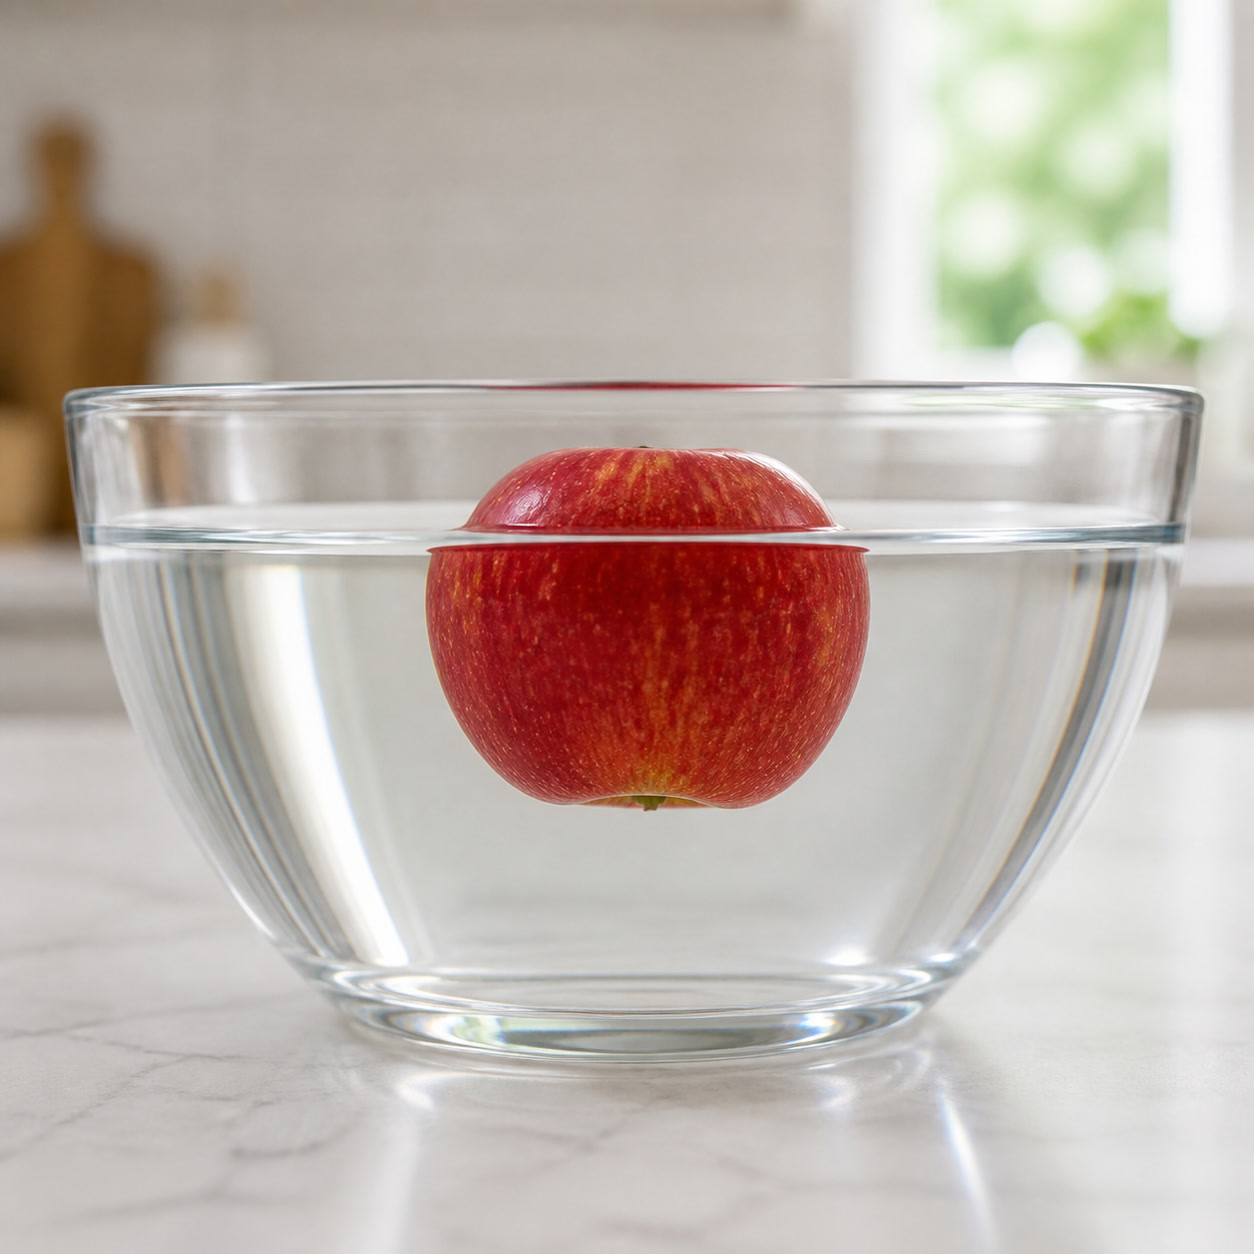
\includegraphics[width=0.42\linewidth]{images/book1/ai/g1-floating-apple.jpg}

{\small Een appel die \omterm{def:g1:floating-and-sinking:words}{drijft} in een kom water: hij ligt diep, met het grootste deel onder het oppervlak --- en toch \omterm{def:g1:floating-and-sinking:words}{drijft} hij.}
\end{omfigure}

\section{Zwaar is niet het hele verhaal}

Veel mensen gokken: ``zware dingen \omterm{def:g1:floating-and-sinking:words}{zinken}, lichte dingen
\omterm{def:g1:floating-and-sinking:words}{drijven}''. Het water heeft een verrassing voor hen.

\begin{example}[De boomstam en het muntje]\label{ex:g1:floating-and-sinking:log}
Een omgevallen boomstam is veel te zwaar om op te tillen --- en toch
\omterm{def:g1:floating-and-sinking:words}{drijft} hij de rivier af. Een klein muntje weegt minder dan een
koekje --- en toch \omterm{def:g1:floating-and-sinking:words}{zinkt} het meteen. Zwaar-of-licht kan dus niet de
hele regel zijn: de reusachtige stam \omterm{def:g1:floating-and-sinking:words}{drijft} terwijl het piepkleine
muntje verdrinkt.
\end{example}

\begin{example}[Het gaat om het materiaal]\label{ex:g1:floating-and-sinking:stuff}
Kijk terug naar het sorteerspel: de plastic lepel dreef en de metalen
lepel zonk, terwijl ze dezelfde vorm hebben en hetzelfde werk doen.
Het verschil zit in het \emph{materiaal} waarvan ze gemaakt zijn ---
hout, kurk en de meeste kunststoffen zijn drijvende materialen;
metaal, steen en glas zijn zinkende materialen. Een ding gedraagt zich
meestal zoals zijn materiaal: hout \omterm{def:g1:floating-and-sinking:words}{drijft}, of het nu een takje is
of een hele stam.
\end{example}

\begin{remark}[Een snufje raadsel]\label{rem:g1:floating-and-sinking:why}
\emph{Waarom} \omterm{def:g1:floating-and-sinking:words}{drijft} hout en \omterm{def:g1:floating-and-sinking:words}{zinkt} metaal? Dat is een echte vraag, en
het volledige antwoord is een van de schatten van deze cursus --- het
heeft ideeën nodig die pas in latere jaren komen. Voorlopig verzamelen
we goede waarnemingen; het ``waarom'' treft ons dan voorbereid aan.
\end{remark}

\section{Het water duwt terug}

\begin{example}[Probeer het: duw de bal onder]\label{ex:g1:floating-and-sinking:push}
Pak in bad een drijvende bal en duw hem met je handpalm langzaam onder
water. Voel je dat? Het water duwt hem terug omhoog, en harder
naarmate je dieper duwt --- en als je hand uitschiet, springt de bal
het water uit. Het water \emph{laat} drijvers niet alleen maar
bovendrijven: het houdt ze actief omhoog, zoals jouw handen een baby
vasthouden.
\end{example}

\begin{omfigure}
\begin{tikzpicture}[scale=0.85]
  \draw[thick] (0,0) -- (0,3.4) (0,0) -- (6.5,0) (6.5,0) -- (6.5,3.4);
  \draw[omDef, thick] (0,2.7) -- (6.5,2.7);
  \fill[omDef, opacity=0.15] (0,0) rectangle (6.5,2.7);
  \draw[thick, fill=white] (3.2,1.5) circle (0.6);
  \node[font=\small] at (3.2,1.5) {bal};
  \draw[-Stealth, very thick, omThm] (3.2,3.3) -- (3.2,2.25);
  \node[right, font=\small, omThm] at (3.35,2.9) {jouw hand duwt omlaag};
  \draw[-Stealth, very thick, omDef] (3.2,0.35) -- (3.2,0.85);
  \node[right, font=\small, omDef] at (3.35,0.55) {het water duwt omhoog};
\end{tikzpicture}

{\small Een bal onder water gehouden: jouw hand duwt omlaag, het water
duwt omhoog. Laat los, en de duw van het water wint.}
\end{omfigure}

\begin{example}[Het bootje van klei]\label{ex:g1:floating-and-sinking:boat}
Rol een klomp boetseerklei tot een bal en laat hem in het water
vallen: hij \omterm{def:g1:floating-and-sinking:words}{zinkt} --- klei is een zinkend materiaal. Neem nu
\emph{dezelfde} klomp en kneed er een schaaltje met hoge randen van,
en zet dat voorzichtig op het water: het \omterm{def:g1:floating-and-sinking:words}{drijft}! Hetzelfde
materiaal, dezelfde klomp --- alleen de vorm is veranderd. Een brede,
holle vorm geeft het water meer om tegenaan te duwen. Dat is het
geheim van de grote schepen: metaal is een zinkend materiaal, maar een
metalen scheepsromp heeft de vorm van een reusachtige holle schaal.
\end{example}

\begin{omfigure}
\begin{tikzpicture}[scale=0.85]
  \draw[thick] (0,0) -- (0,2.6) (0,0) -- (4.6,0) (4.6,0) -- (4.6,2.6);
  \draw[omDef, thick] (0,2.0) -- (4.6,2.0);
  \fill[omDef, opacity=0.15] (0,0) rectangle (4.6,2.0);
  \fill[omThm] (2.3,0.35) circle (0.35);
  \node[below, font=\small] at (2.3,-0.2) {kleibal: zinkt};
  \draw[thick] (6.4,0) -- (6.4,2.6) (6.4,0) -- (11,0)
    (11,0) -- (11,2.6);
  \draw[omDef, thick] (6.4,2.0) -- (11,2.0);
  \fill[omDef, opacity=0.15] (6.4,0) rectangle (11,2.0);
  \draw[thick, omThm, fill=white]
    (7.9,2.25) -- (8.1,1.75) -- (9.3,1.75) -- (9.5,2.25);
  \node[below, font=\small] at (8.7,-0.2) {dezelfde klomp als schaaltje: drijft};
\end{tikzpicture}

{\small Eén klomp klei, twee vormen, twee lotgevallen. De holle
schaalvorm geeft het water meer om omhoog te houden.}
\end{omfigure}

\section{Oefeningen}

\begin{exercise}[$\star$]\label{exo:g1:floating-and-sinking:1}
Sorteer in drijvers en zinkers: een kurk; \ een sleutel; \ een droog
takje; \ een knikker; \ een plastic eendje; \ een steen.
\end{exercise}

\begin{exercise}[$\star$]\label{exo:g1:floating-and-sinking:2}
Waarom moet je in \cref{met:g1:floating-and-sinking:test} het voorwerp
voorzichtig op het water leggen in plaats van het erin te gooien?
\end{exercise}

\begin{exercise}[$\star$]\label{exo:g1:floating-and-sinking:3}
Nora gokt vóór de proef: ``De metalen lepel zal \omterm{def:g1:floating-and-sinking:words}{drijven}, want lepels
\omterm{def:g1:floating-and-sinking:words}{drijven}.'' Wat gebeurde er in het sorteerspel? Waar moet Nora naar
kijken in plaats van naar waar de vorm voor dient: naar het materiaal
of naar de naam?
\end{exercise}

\begin{exercise}[$\star$]\label{exo:g1:floating-and-sinking:4}
Noem één ding dat zwaar is en \omterm{def:g1:floating-and-sinking:words}{drijft}, en één ding dat \omterm{def:g1:light-and-shadows:source}{licht} is en
\omterm{def:g1:floating-and-sinking:words}{zinkt}. Wat laat dit zien over de gok ``zware dingen
\omterm{def:g1:floating-and-sinking:words}{zinken}''?
\end{exercise}

\begin{exercise}[$\star$]\label{exo:g1:floating-and-sinking:5}
Een takje \omterm{def:g1:floating-and-sinking:words}{drijft}. Zal een hele boomstam ook \omterm{def:g1:floating-and-sinking:words}{drijven}? Welk voorbeeld
uit het hoofdstuk helpt je bij het antwoord?
\end{exercise}

\begin{exercise}[$\star$]\label{exo:g1:floating-and-sinking:6}
Duw in bad een drijvende bal onder water en laat hem dan los. Wat voel
je terwijl je duwt, en wat doet de bal als je loslaat?
\end{exercise}

\begin{exercise}[$\star$]\label{exo:g1:floating-and-sinking:7}
Schepen zijn van metaal gemaakt, en metaal is een zinkend materiaal.
Welke vorm redt het schip? Welke proef uit het hoofdstuk laat dat
zien?
\end{exercise}

\begin{exercise}[$\star$]\label{exo:g1:floating-and-sinking:8}
Onderzoek het in bad: \omterm{def:g1:floating-and-sinking:words}{drijft} of \omterm{def:g1:floating-and-sinking:words}{zinkt} een volle, dichtgedraaide fles
water? En diezelfde fles leeg, met de dop erop? Zeg eerst je gokken,
en probeer het dan.
\end{exercise}

\begin{exercise}[$\star\star$]\label{exo:g1:floating-and-sinking:9}
Het kleibootje van Leo \omterm{def:g1:floating-and-sinking:words}{drijft} prima --- tot hij het weer tot een bal
platdrukt, en het \omterm{def:g1:floating-and-sinking:words}{zinkt}. ``Het water werd moe van het vasthouden,''
zegt Leo. Geef een betere verklaring, met behulp van
\cref{ex:g1:floating-and-sinking:boat}.
\end{exercise}
